%=======================+=========================
%================   Detector Overview ================
%=================================================

%\section[Detector overview (Curtis)]{Detector overview
\section[Detector overview]{Detector overview \label{sec:overview}}
The design of the GlueX detector \cite{Ghoul:2015ifw} is based on a solenoidal magnet that surrounds all detectors in the central region, providing a magnetic field of about $2$~T along the direction of the photon beam, which impinges on a 
$30$~cm-long\textcolor{blue}{(There was a question on the length of the target. Target section shows 30cm, but is it 29.25cm?)} liquid hydrogen target.  A schematic of the detector including its major sub-detectors is given in Fig.\,\ref{fig:layout_spectrometer}.

% ======================================================================================

\begin{figure*}[!htb]
\centering
  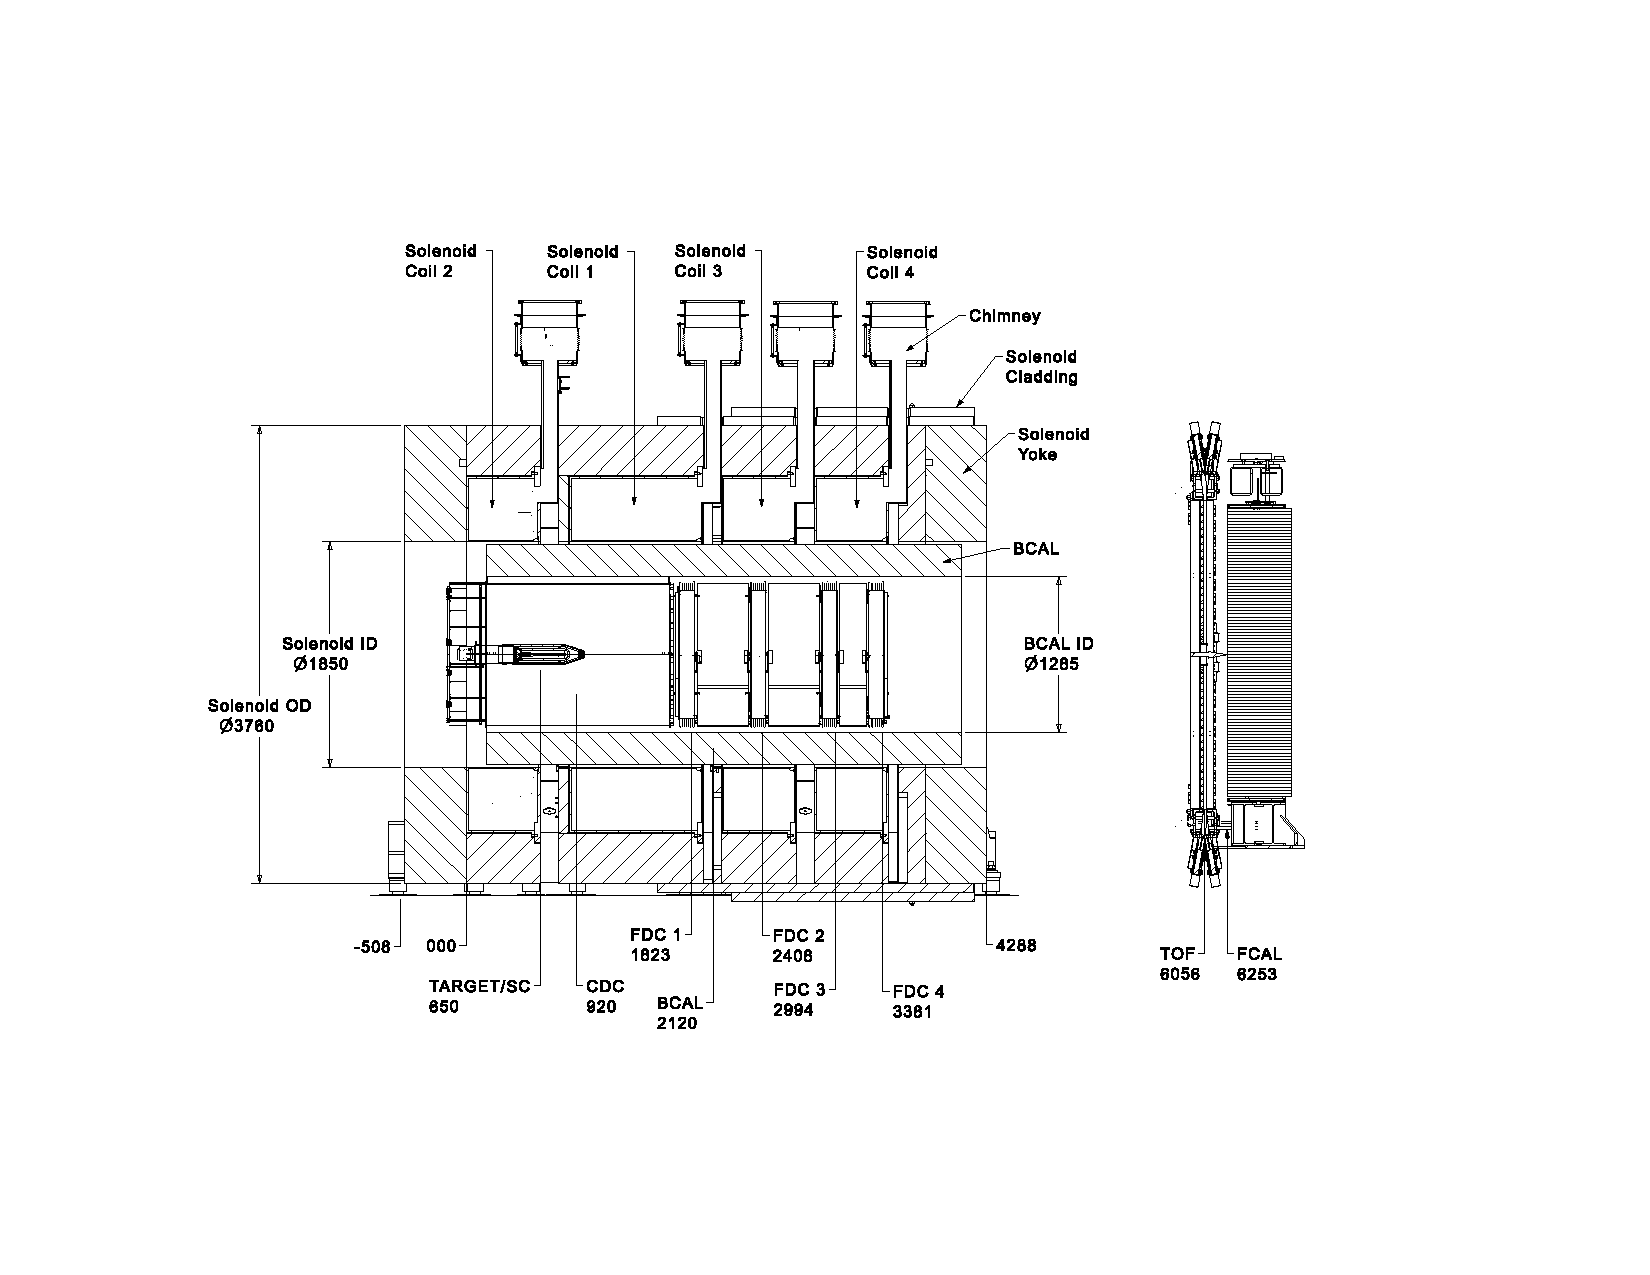
\includegraphics[angle=0,viewport=95 115 628 500,clip,width=1.0\linewidth]{figures/gluex_spectrometer_drawing_01_bw}%
  \caption[layout]{GlueX spectrometer layout. Dimensions are given in mm. The
    numbers show the Z-coordinates of the detectors' centers, or of
    the front face of the calorimeter modules in case of the FCAL.
    Glossary: 
              SC  - Start Counter (Section \ref{sec:st}), 
              CDC - Central Drift Chamber (Section \ref{sec:cdc}), 
              FDC - Forward Drift Chamber (Section \ref{sec:fdc}),
              BCAL - Barrel Calorimeter (Section \ref{sec:bcal}), 
              TOF -  Time-of-Flight hodoscope (Section \ref{sec:tof}), 
              FCAL - Forward Calorimeter (Section \ref{sec:fcal}).
%
%    \begin{tabular}{lll}
%       Name  & Detector & Section \\ \hline
%              SC  & Start Counter & \ref{sec:st} \\ 
%              CDC & Central Drift Chamber  & \ref{sec:cdc} \\ 
%              FDC & Forward Drift Chamber  & \ref{sec:fdc} \\ 
%              BCAL & Barrel Calorimeter    & \ref{sec:bcal} \\ 
%              TOF &  Time-of-Flight hodoscope & \ref{sec:tof} \\ 
%              FCAL & Forward Calorimeter    & \ref{sec:fcal} \\ 
%    \end{tabular}
    \label{fig:layout_spectrometer}
  }
\end{figure*}

% ======================================================================================

%\begin{figure}[tbp]
%\begin{center}
%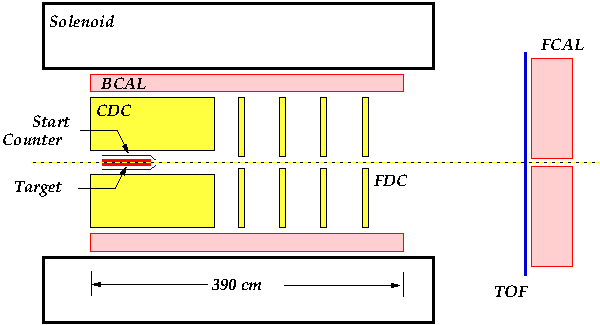
\includegraphics[width=0.7\textwidth]{figures/GlueX_Sketch.pdf}  
%\caption{\label{fig:gluexsketch}          
%  Sketch of GlueX detector.  The main systems of the detector are the Start %Counter \cite{Pooser:2019rhu}, the Central Drift Chamber (CDC) %\cite{VanHaarlem:2010yq} the Forward Drift Chamber (FDC) \cite{Pentchev2017281}, %a scintillator-based Time of Flight (TOF) wall and a lead-glass Forward %Calorimeter (FCAL) \cite{MORIYA201360}. The Barrel Calorimeter (BCAL) is %sandwiched between the drift chambers and the inner radius of the solenoid.  %(Color online)
%}   
%\end{center}  
%\end{figure}
